\section{Fourier Transform Properties}


\begin{frame}{Fourier Transform: Recall}
Synthesis equation:
    \begin{equation}
        x(t) = \frac{1}{2\pi}\int_{-\infty}^{\infty}X(j\omega)e^{j\omega t} d\omega.
    \end{equation}
Analysis equation:
    \begin{equation}
        X(j\omega) = \int_{-\infty}^{\infty}x(t)e^{-j\omega t} dt.
    \end{equation}

    \begin{equation}
        x(t) \overset{\mathcal{F}}{\longleftrightarrow} X(j\omega).
    \end{equation}
\end{frame}


\begin{frame}{Linearity}
    If
    \begin{equation*}
        x(t) \overset{\mathcal{F}}{\longleftrightarrow} X(j\omega).
    \end{equation*}
    and
    \begin{equation*}
        y(t) \overset{\mathcal{F}}{\longleftrightarrow} Y(j\omega).
    \end{equation*}
    then

    \mode<beamer>
    {
    \begin{equation*}
        ax(t) + by(t) \overset{\mathcal{F}}{\longleftrightarrow} \pause aX(j\omega)+ bY(j\omega).
    \end{equation*}
    }
\end{frame}



\begin{frame}{Time Shifting}
    If
    \begin{equation*}
        x(t) \overset{\mathcal{F}}{\longleftrightarrow} X(j\omega).
    \end{equation*}
    then

    \mode<beamer>
    {
    \begin{equation*}
        x(t-t_0) \overset{\mathcal{F}}{\longleftrightarrow} \pause e^{-j\omega t_0}X(j\omega).
    \end{equation*}
    }
\end{frame}

\begin{frame}[plain]{Proof}
    \mode<beamer>
    {
        \begin{align*}
          x(t) &= \frac{1}{2\pi}\int_{-\infty}^{\infty}X(j\omega)e^{j\omega t} d\omega.\\
          x(t - t_0) &= \frac{1}{2\pi}\int_{-\infty}^{\infty}X(j\omega)e^{j\omega (t-t_0)} d\omega.\\
           &= \frac{1}{2\pi}\int_{-\infty}^{\infty}\left(e^{-j\omega t_0}X(j\omega)\right)e^{j\omega t} d\omega.\\
        \end{align*}
        \pause
        This is the synthesis equation for $x(t-t_0)$. Therefore,
        \begin{equation*}
            \mathcal{F}\{x(t-t_0)\} = e^{-j\omega t_0}X(j\omega).
        \end{equation*}
        Magnitude of the Fourier transform not altered. Time shift introduces a phase shift $-\omega t_0$, which is a linear function of $\omega$.
    }
\end{frame}

\begin{frame}
    \begin{columns}
        \column{0.6\textwidth}
            \begin{example}
            Evaluate the Fourier transform of $x(t)$.
                \begin{figure}
                \centering
                    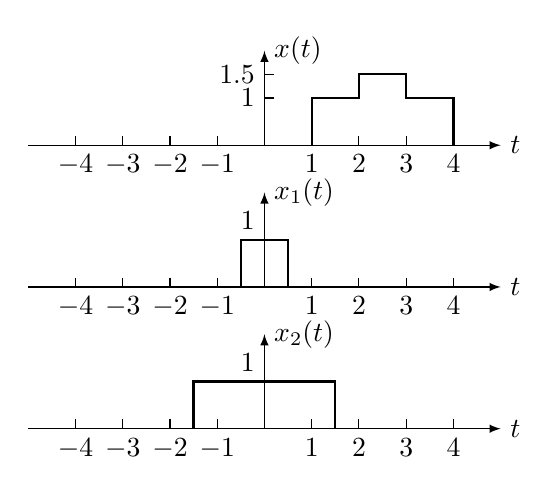
\begin{tikzpicture}[scale=0.6]
	\begin{scope}
		\def\xmin{-5}
		\def\xmax{5}
		\def\ymin{0}
		\def\ymax{2}
		
		\draw[-latex] (\xmin, 0) -- (\xmax, 0) node[anchor=west] {$t$};
		\draw[-latex] (0, \ymin) -- (0, \ymax) node[anchor=west] {$x(t)$};
		
		\foreach \x in {-4, -3, -2, -1, 1, 2, 3, 4}
		{
			\draw (\x, 0.2) -- ++(0, -0.2) node[anchor=north] {$\x$};
		}
		\foreach \y in {1, 1.5}
		{
			\draw (0.2,  \y) -- ++(-0.2, 0) node[anchor=east] {$\y$};
		}	
		\draw[thick] (1,0) |- (2, 1) |- (3,1.5) |- (4,1) -- (4,0);	
	\end{scope}
\pause
	\begin{scope}[yshift=-3cm]
		\def\xmin{-5}
		\def\xmax{5}
		\def\ymin{0}
		\def\ymax{2}
		
		\draw[-latex] (\xmin, 0) -- (\xmax, 0) node[anchor=west] {$t$};
		\draw[-latex] (0, \ymin) -- (0, \ymax) node[anchor=west] {$x_1(t)$};
		
		\foreach \x in {-4, -3, -2, -1, 1, 2, 3, 4}
		{
			\draw (\x, 0.2) -- ++(0, -0.2) node[anchor=north] {$\x$};
		}
		
		
		\node at (0,1) [anchor=south east] {$1$};		
		
		\draw[thick] (-0.5,0) |- (0.5, 1) -- (0.5, 0);	
	\end{scope}
	\begin{scope}[yshift=-6cm]
		\def\xmin{-5}
		\def\xmax{5}
		\def\ymin{0}
		\def\ymax{2}
		
		\draw[-latex] (\xmin, 0) -- (\xmax, 0) node[anchor=west] {$t$};
		\draw[-latex] (0, \ymin) -- (0, \ymax) node[anchor=west] {$x_2(t)$};
		
		\foreach \x in {-4, -3, -2, -1, 1, 2, 3, 4}
		{
			\draw (\x, 0.2) -- ++(0, -0.2) node[anchor=north] {$\x$};
		}
		
		
		\node at (0,1) [anchor=south east] {$1$};		
		
		\draw[thick] (-1.5,0) |- (1.5, 1) -- (1.5, 0);	
	\end{scope}
\end{tikzpicture} 
                \end{figure}
            \end{example}
        \column{0.4\textwidth}
        \pause
        \mode<beamer>
        {
            \begin{equation*}
                \begin{aligned}
                    x(t) &= \frac{1}{2}x_1(t-2.5) + x_2(t-2.5)\\
                    X_1(j\omega) &= \frac{2\sin(\omega/2)}{\omega}\\
                    X_2(j\omega) &= \frac{2\sin(3\omega/2)}{\omega}\\
                \end{aligned}
            \end{equation*}
            \pause
            \begin{equation*}
                X(j\omega) = e^{-j5\omega/2}\left[\frac{\sin(\omega/2) + 2\sin(3\omega/2)}{\omega}\right].
            \end{equation*}
        }
    \end{columns}

\end{frame}


\begin{frame}{Conjugation and Conjugate Symmetry}
    If
    \begin{equation*}
        x(t)  \overset{\mathcal{F}}{\longleftrightarrow}  X(j\omega).
    \end{equation*}
    then
    \begin{equation*}
        x^\ast(t)  \overset{\mathcal{F}}{\longleftrightarrow}  X^\ast(-j\omega).
    \end{equation*}
    \pause
    \mode<beamer>
    {
        \begin{columns}
            \column{0.5\textwidth}
                \begin{align*}
                    X^\ast(j\omega) &= \left[\int_{-\infty}^{\infty}x(t)e^{-j\omega t} dt \right]^\ast\\
                    &= \int_{-\infty}^{\infty}x^\ast(t)e^{j\omega t} dt\\
                    \text{Replacing $\omega$ by $-\omega$ }\\
                    X^\ast(-j\omega) &= \int_{-\infty}^{\infty}x^\ast(t)e^{-j\omega t} dt\\
                \end{align*}
                which is the analysis equation for $x^\ast(t)$.\\
                \pause
            \column{0.5\textwidth}
                If $x(t)$ is real, i.e., $x(t) = x^\ast(t)$, $X(j\omega)$ has conjugate symmetry.
                \begin{equation*}
                    X(-j\omega) = X^\ast(j\omega)\quad [x(t) \text{ real}]
                \end{equation*}

        \end{columns}



    }


\end{frame}

\begin{frame}{Using Conjugate Symmetry}
    Use the conjugate property to comment about the symmetry of \ft~of a signal $x(t)$ if
    \begin{enumerate}
        \item $x(t)$ is real,
        \item $x(t)$ is real and even, and
        \item $x(t)$ is real and odd.
    \end{enumerate}
\end{frame}

\begin{frame}
    Expressing $X(j\omega)$ in rectangular form as
    \begin{equation*}
        X(j\omega)
        = \mathfrak{Re}\left\{X(j\omega)\right\} + j\mathfrak{Im}\left\{X(j\omega)\right\},
    \end{equation*}
   % \pause
    then if $x(t)$ is real [$x(t) = x^\ast(t)$]
    \begin{align*}
        \mathfrak{Re}\left\{X(j\omega)\right\} &= \mathfrak{Re}\left\{X(-j\omega)\right\}\quad \text{and}\\
        \mathfrak{Im}\left\{X(j\omega)\right\} &= -\mathfrak{Im}\left\{X(-j\omega)\right\}\\
    \end{align*}
That is, the real part of the Fourier transform is an even function of frequency, and the imaginary part is an odd function of frequency.
\pause
Considering
    \begin{equation*}
        X(j\omega) = |X(j\omega)|e^{\angle X(j\omega)},
    \end{equation*}
    we see that $|X(j\omega)|$ is an even function of frequency, and $\angle X(j\omega)$ is an odd function of frequency.


\end{frame}

\begin{frame}
    If $x(t)$ is both real and even, then $X(j\omega)$ will also be real and even.\par
    \noindent{\bf Proof}:\par
\mode<beamer>
{
    \begin{equation*}
        X(-j\omega) = \int_{-\infty}^{\infty} x(t)e^{j\omega t}dt
    \end{equation*}
    \pause
    With the substitution $\tau = -t$
    \begin{equation*}
        X(-j\omega) = \int_{-\infty}^{\infty} x(-\tau)e^{-j\omega \tau}d\tau
    \end{equation*}
    Since $x(-\tau) = x(\tau)$ we have
    \begin{equation*}
        X(-j\omega) = \int_{-\infty}^{\infty} x(\tau)e^{j\omega \tau}d\tau
    \end{equation*}

    \begin{equation*}
        X(-j\omega) = X(j\omega)
    \end{equation*}
    In a similar manner, it can be shown that if $x(t)$ is a real and odd function of time, so that $x(t) = - x(- t)$, then $X(j\omega)$ is purely imaginary and odd.

}
\end{frame}


\begin{frame}{Fourier Transforms of Odd and Even Parts}
    A real function $x(t)$ can be expressed as
    \begin{equation*}
        x(t) = x_e(t) + x_o(t),
    \end{equation*}
    where $x_e(t) = \mathfrak{Ev}\left\{x(t)\right\}$ is the even part of $x(t)$ and $x_o(t) = \mathfrak{Od}\left\{x(t)\right\}$ is the odd part of $x(t)$. Express Fourier transforms of
    \begin{enumerate}
      \item $x_e(t) = \mathfrak{Ev}\left\{x(t)\right\}$, and
      \item $x_o(t) = \mathfrak{Od}\left\{x(t)\right\}$.
    \end{enumerate}
    in terms of $X(j\omega)$.
\end{frame}

\begin{frame}
    \mode<beamer>
    {
        From the linearity of the Fourier transform,
        \begin{equation*}
            \mathfrak{F}\left\{x(t)\right\} = \mathfrak{F}\left\{x_e(t)\right\} +\mathfrak{F}\left\{x_o(t)\right\},
        \end{equation*}
        and from the preceding discussion, $\mathfrak{F}\left\{x_e(t)\right\}$ is a real function and $\mathfrak{F}\left\{x_o(t)\right\}$ is purely imaginary. Thus, we can conclude that, with $x(t)$ real,
        \pause
        \begin{align*}
            x(t) &\overset{\mathcal{F}}{\longleftrightarrow} X(j\omega),\\
            \mathfrak{Ev}\left\{x(t)\right\} &\overset{\mathcal{F}}{\longleftrightarrow} \mathfrak{Re}\left\{X(j\omega)\right\},\\
            \mathfrak{Od}\left\{x(t)\right\} &\overset{\mathcal{F}}{\longleftrightarrow} j\mathfrak{Im}\left\{X(j\omega)\right\}.
        \end{align*}
    }
\end{frame}


\begin{frame}{Example}
    Use the symmetry properties of the Fourier transform to evaluate the Fourier transform of
    \begin{equation*}
        x(t) = e^{-a|t|}, \quad a>0.
    \end{equation*}
    \pause
    \begin{columns}
        \column{0.5\textwidth}
            We have already found that
            \begin{equation*}
                e^{-at} \overset{\mathcal{F}}{\longleftrightarrow} \frac{1}{a+j\omega}.
            \end{equation*}

            \begin{align*}
                x(t) &= e^{-a|t|} = e^{-at}u(t) + e^{at}u(-t)\\
                &= 2\left[\frac{e^{-at}u(t) + e^{at}u(-t)}{2}\right]\\
                &= 2\mathfrak{Ev}\left\{ e^{-at}u(t)\right\}.
            \end{align*}

        \column{0.5\textwidth}
            Since $e^{-at}u(t)$is real valued, the symmetry properties of the Fourier transform lead us to conclude that
            \begin{equation*}
                \mathfrak{Ev}\left\{ e^{-at}u(t)\right\} \overset{\mathcal{F}}{\longleftrightarrow} \mathfrak{Re}\left\{ \frac{1}{a+j\omega}\right\}.
            \end{equation*}
            \pause
            \begin{equation*}
                X(j\omega) = 2\mathfrak{Re}\left\{ \frac{1}{a+j\omega}\right\} = \frac{2a}{a^2 + \omega^2}.
            \end{equation*}
    \end{columns}
\end{frame}


\begin{frame}{Differentiation and Integration}
    Synthesis equation:
    \begin{equation*}
        x(t) = \frac{1}{2\pi}\int_{-\infty}^{\infty}X(j\omega)e^{j\omega t} d\omega.
    \end{equation*}
    Differentiating both  sides of the equation
    \begin{equation*}
        \frac{dx(t)}{dt} = \frac{1}{2\pi}\int_{-\infty}^{\infty}j\omega X(j\omega)e^{j\omega t} d\omega.
    \end{equation*}
    Therefore,
    \begin{equation*}
        \frac{dx(t)}{dt}  \overset{\mathcal{F}}{\longleftrightarrow}  j\omega X(j\omega).
    \end{equation*}
    Integration:
    \begin{equation*}
        \int_{-\infty}^{t} x(\tau)d\tau \overset{\mathcal{F}}{\longleftrightarrow} \frac{1}{ j\omega} X(j\omega) + \pi X(0)\delta(\omega).
    \end{equation*}
\end{frame}


\begin{frame}[plain]
    \begin{example}
        Determine the Fourier transform of the unit step $x(t) = u(t)$ making use of the knowledge that
    \begin{equation*}
        g(t) = \delta(t)  \overset{\mathcal{F}}{\longleftrightarrow} G(j\omega) = 1.
    \end{equation*}
    \end{example}
    \pause
    \begin{columns}
        \column{0.6\textwidth}
        \mode<beamer>
        {
            Noting that
            \begin{equation*}
                x(t) = \int_{-\infty}^{t} g(\tau)d\tau
            \end{equation*}
            we obtain that
            \begin{equation*}
                X(j\omega) = \frac{1}{ j\omega} G(j\omega) + \pi G(0)\delta(\omega).
            \end{equation*}
            Since $G(j\omega) = 1$
            \begin{equation*}
                X(j\omega) = \frac{1}{ j\omega}  + \pi\delta(\omega).
            \end{equation*}
        }
        \column{0.4\textwidth}
        \pause
        \mode<beamer>
        {
            Observe that, we can apply the differentiation property to recover the transform of the impulse:
            \begin{equation*}
                \delta(t) = \frac{du(t)}{dt}\overset{\mathcal{F}}{\longleftrightarrow} j\omega\left[ \frac{1}{ j\omega}  + \pi\delta(\omega)\right] = 1.
            \end{equation*}
            Note: $\omega \delta(\omega) = 0$
        }
    \end{columns}
\end{frame}

\begin{frame}[plain]
    \begin{columns}
        \column{0.6\textwidth}
        \begin{example}
            Determine the Fourier transform of the signal $x(t)$ shown below:
            \begin{figure}
            \centering
                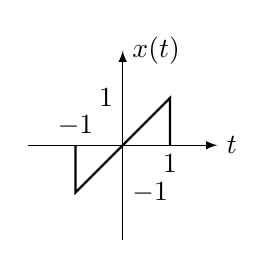
\begin{tikzpicture}[scale=0.6]
	\begin{scope}
		\def\xmin{-2}
		\def\xmax{2}
		\def\ymin{-2}
		\def\ymax{2}
		
		\draw[-latex] (\xmin, 0) -- (\xmax, 0) node[anchor=west] {$t$};
		\draw[-latex] (0, \ymin) -- (0, \ymax) node[anchor=west] {$x(t)$};
		\node at (-1,0) [anchor=south] {$-1$};
		\node at (1,0) [anchor=north] {$1$};		
		
		\node at (0,-1) [anchor=west] {$-1$};
		\node at (0,1) [anchor=east] {$1$};			

		\draw[thick] (-1,0) -- (-1, -1) -- (1,1) -- (1,0);	
	\end{scope}
\end{tikzpicture}
            \end{figure}
        \end{example}
        \pause

        \mode<beamer>
        {
            \begin{figure}
            \centering
                \begin{tikzpicture}[scale=0.6]
	\begin{scope}
		\def\xmin{-2}
		\def\xmax{2}
		\def\ymin{-1}
		\def\ymax{2}
		
		\node at (-4, 0) {$g(t) = \frac{dx(t)}{dt}=$};
		
		\draw[-latex] (\xmin, 0) -- (\xmax, 0) node[anchor=west] {$t$};
		\draw[-latex] (0, \ymin) -- (0, \ymax) node[anchor=south] {$$};
		\node at (-1,0) [anchor=north] {$-1$};
		\node at (1,0) [anchor=north] {$1$};		
		

		\node at (0,1) [anchor=south east] {$1$};			

		\draw[thick] (-1,0) -- (-1, 1) -- (1,1) -- (1,0);	
	\end{scope}
	
	\begin{scope}[xshift=5.5cm]
		\def\xmin{-2}
		\def\xmax{2}
		\def\ymin{-2}
		\def\ymax{2}
		
		\node at (-2.5, 0) {$+$};
		
		\draw[-latex] (\xmin, 0) -- (\xmax, 0) node[anchor=west] {$t$};
		\draw[-latex] (0, \ymin) -- (0, \ymax) node[anchor=south] {$$};
		\node at (-1,0) [anchor=south] {$-1$};
		\node at (1,0) [anchor=south] {$1$};		
		

			

		\draw[thick, -latex] (-1,0) -- ++(0, -1)  node[anchor=north] {$-1$};	

		\draw[thick, -latex] (1,0) -- ++(0, -1)  node[anchor=north] {$-1$};				
	\end{scope}	
\end{tikzpicture}
            \end{figure}
        }
        \column{0.4\textwidth}
        \pause
        \mode<beamer>
        {
            \begin{equation*}
                G(j\omega) = \left(\frac{2\sin \omega}{\omega}\right) - e^{j\omega} - e^{-j\omega}
            \end{equation*}
            \pause
            \begin{equation*}
                X(j\omega) = \frac{1}{ j\omega} G(j\omega) + \pi G(0)\delta(\omega).
            \end{equation*}
            As $G(0) = 0$\\
            \pause
            \begin{equation*}
                X(j\omega) = \frac{2\sin \omega}{ j\omega^2}  - \frac{2\cos \omega}{j\omega}
            \end{equation*}
            Note: $ X(j\omega)$ is purely imaginary and odd.
        }
    \end{columns}
\end{frame}


\begin{frame}{Time and Frequency Scaling}
    If
    \begin{equation*}
        x(t)  \overset{\mathcal{F}}{\longleftrightarrow}  X(j\omega).
    \end{equation*}
    then
    \begin{equation*}
        x(at)  \overset{\mathcal{F}}{\longleftrightarrow}  \frac{1}{|a|}X\left(\frac{j\omega}{a}\right).
    \end{equation*}
    where $a$ is a real constant.\pause \\
    Letting $a = -1$\pause
    \begin{equation*}
        x(-t)  \overset{\mathcal{F}}{\longleftrightarrow}  X(-j\omega).
    \end{equation*}
    The scaling property is another example of the inverse relationship between time and frequency.
\end{frame}



\begin{frame}{Duality}
    Because of the similarity between the synthesis equation
    \begin{equation}
        x(t) = \frac{1}{2\pi}\int_{-\infty}^{\infty}X(j\omega)e^{j\omega t} d\omega.
    \end{equation}
    and the analysis equation,
    \begin{equation}
        X(j\omega) = \int_{-\infty}^{\infty}x(t)e^{-j\omega t} dt.
    \end{equation}
    for any transform pair, there is a dual pair with the time and frequency variables interchanged.
\end{frame}

\begin{frame}

        We determined the Fourier transform of the square pulse as
        \begin{equation*}
            x_1(t) = \begin{cases}
                1,& |t| < T_1,\\
                0, & |t| > T_1,
            \end{cases}
             \overset{\mathcal{F}}{\longleftrightarrow}
             X_1(j\omega) = \frac{2\sin \omega T_1}{\omega}
        \end{equation*}

        \begin{figure}
          \centering
          \begin{tikzpicture}[scale=0.5]
\begin{scope}[xshift=-6cm, yshift=2cm]

	\def\xmin{-4}
	\def\xmax{4}
	\def\ymin{0}
	\def\ymax{2}
	\def\period{2.0}
	\def\T1{1}
	\def\A{1}
	
	\edef\pulse{|- ++(2*\T1, \A) |- ++( \period - \T1, -\A)}

	
	\draw (\xmin-1, 0) --(\xmax+1, 0) node[anchor=west] {\small $t$};
	\draw (0, \ymin) --(0, \ymax) node[anchor=south] {\small $x_1(t)$};
	\draw[thick] (-3, 0) -- (-\T1,0) -- (-\T1, 1) -- (\T1,1) -- (\T1,0) -- (3,0);
		
		\node at (-\T1, 0) [anchor=north] {\small $-T_1$};
		\node at (\T1, 0) [anchor=north] {\small $T_1$};
		\node at (0, 1) [anchor=south east] {\small $1$};

\end{scope}		
\begin{scope}	
    \begin{axis}[
		y=4cm,
		x=1cm,
		 clip=false,
		 xmin=-5.5,xmax=5.5,
		 xlabel= $\omega$,
		 ylabel={$X_1(j\omega)$},
		 ymin=-0.5,ymax=1.2,
		 axis lines=middle,
         	%xtick={-5, -4, ..., 5},
		 %ytick={-1, 1},
		 yticklabels=\empty,
		 xticklabels=\empty,
		 every axis x label/.style={at={(ticklabel* cs:1.05)}, anchor=west,},
		every axis y label/.style={at={(ticklabel* cs:1.05)}, anchor=south,},
     ]
		%\addplot+[red, smooth, mark=none] table [x={n}, y={xn}] {periodic_square_fs_samples_of_envilope_gen.dat};
		\addplot [red, thick, domain=-5:5, samples=200] plot{sin(pi*deg(x))/(pi*x)};
		\node at (axis cs:0, 1) [anchor=east] { $2T_1$ };
		\draw[latex-] (axis cs:pi/3, 0) --(axis cs:0.6,-0.3) node  [anchor=north] { $\pi/T_1$ } ;
		\draw[latex-] (axis cs:-pi/3, 0) --(axis cs:-0.6,-0.3) node  [anchor=north] { $-\pi/T_1$ } ;		
    \end{axis}
\end{scope}		
\end{tikzpicture}

          \caption{Rectangular pulse and the Fourier transform.}\label{fi:square_pulse}
        \end{figure}

\end{frame}


\begin{frame}
        We also determined that for a time-domain signal that is similar in shape to the $X_1(j\omega)$ as
        \begin{equation*}
        x_2(t) = \frac{\sin W t}{\pi t}
         \overset{\mathcal{F}}{\longleftrightarrow}
            X_2(j\omega) = \begin{cases}
                1,& |\omega| < W,\\
                0, & |\omega| > W.
            \end{cases}
        \end{equation*}
        \begin{figure}
          \centering
          \begin{tikzpicture}
\begin{scope}	
    \begin{axis}[
		y=2cm,
		x=0.5cm,
		 clip=false,
		 xmin=-5.5,xmax=5.5,
		 xlabel= $t$,
		 ylabel={$x_2(t)$},
		 ymin=-0.5,ymax=1.2,
		 axis lines=middle,
         	%xtick={-5, -4, ..., 5},
		 %ytick={-1, 1},
		 yticklabels=\empty,
		 xticklabels=\empty,
		 every axis x label/.style={at={(ticklabel* cs:1.05)}, anchor=west,},
		every axis y label/.style={at={(ticklabel* cs:1.05)}, anchor=south,},
     ]
		%\addplot+[red, smooth, mark=none] table [x={n}, y={xn}] {periodic_square_fs_samples_of_envilope_gen.dat};
		\addplot [red, thick, domain=-5:5, samples=200] plot{sin(pi*deg(x))/(pi*x)};
		\node at (axis cs:0, 1) [anchor=east] { $W/\pi$ };
		\draw[latex-] (axis cs:pi/3, 0) --(axis cs:pi/3,-0.3) node  [anchor=north] { $\pi/W$ } ;
		\draw[latex-] (axis cs:-pi/3, 0) --(axis cs:-pi/3,-0.3) node  [anchor=north] { $-\pi/W$ } ;		
    \end{axis}
\end{scope}	
\begin{scope}[xshift=10cm, yshift=1cm]

	\def\xmin{-2}
	\def\xmax{2}
	\def\ymin{0}
	\def\ymax{2}
	\def\period{2.0}
	\def\T1{0.5}
	\def\A{0.5}
	
	\edef\pulse{|- ++(2*\T1, \A) |- ++( \period - \T1, -\A)}

	
	\draw (\xmin-1, 0) --(\xmax+1, 0) node[anchor=west] {\small $\omega$};
	\draw (0, \ymin) --(0, \ymax) node[anchor=south] {\small $X_2(j\omega)$};
	\draw[thick] (-3, 0) -- (-\T1,0) -- (-\T1, 1) -- (\T1,1) -- (\T1,0) -- (3,0);
		
		\node at (-\T1, 0) [anchor=north] {\small $-W$};
		\node at (\T1, 0) [anchor=north] {\small $W$};
		\node at (0, 1) [anchor=south east] {\small $1$};

\end{scope}

\end{tikzpicture} 
          \caption{Fourier transform for $x(t)$.}\label{fi:xomega_square}
        \end{figure}
\end{frame}



\begin{frame}[plain]
\mode<beamer>
{
        \begin{figure}
          \centering
          \begin{tikzpicture}
\begin{scope}[xshift=0cm, yshift=0cm]

	\def\xmin{-2}
	\def\xmax{2}
	\def\ymin{0}
	\def\ymax{2}
	\def\period{2.0}
	\def\T1{0.5}
	\def\A{0.5}
	
	\edef\pulse{|- ++(2*\T1, \A) |- ++( \period - \T1, -\A)}

	
	\draw (\xmin-1, 0) --(\xmax+1, 0) node[anchor=west] {\small $t$};
	\draw (0, \ymin) --(0, \ymax) node[anchor=south] {\small $x_1(t)$};
	\draw[thick] (-3, 0) -- (-\T1,0) -- (-\T1, 1) -- (\T1,1) -- (\T1,0) -- (3,0);
		
		\node at (-\T1, 0) [anchor=north] {\small $-T_1$};
		\node at (\T1, 0) [anchor=north] {\small $T_1$};
		\node at (0, 1) [anchor=south east] {\small $1$};
\end{scope}		
%\pause
\begin{scope}[xshift=5cm, yshift=-1cm]	
    \begin{axis}[
		y=2cm,
		x=0.5cm,
		 clip=false,
		 xmin=-5.5,xmax=5.5,
		 xlabel= $\omega$,
		 ylabel={$X_1(j\omega)$},
		 ymin=-0.5,ymax=1.2,
		 axis lines=middle,
         	%xtick={-5, -4, ..., 5},
		 %ytick={-1, 1},
		 yticklabels=\empty,
		 xticklabels=\empty,
		 every axis x label/.style={at={(ticklabel* cs:1.05)}, anchor=west,},
		every axis y label/.style={at={(ticklabel* cs:1.05)}, anchor=south,},
     ]
		%\addplot+[red, smooth, mark=none] table [x={n}, y={xn}] {periodic_square_fs_samples_of_envilope_gen.dat};
		\addplot [red, thick, domain=-5:5, samples=200] plot{sin(pi*deg(x))/(pi*x)};
		\node at (axis cs:0, 1) [anchor=east] { $2T_1$ };
		\draw[latex-] (axis cs:pi/3, 0) --(axis cs:pi/3,-0.3) node  [anchor=north] { $\pi/T_1$ } ;
		\draw[latex-] (axis cs:-pi/3, 0) --(axis cs:-pi/3,-0.3) node  [anchor=north] { $-\pi/T_1$ } ;		
    \end{axis}
\end{scope}		

%\pause

\begin{scope}[xshift=-2.7cm, yshift=-6cm]
    \begin{axis}[
		y=2cm,
		x=0.5cm,
		 clip=false,
		 xmin=-5.5,xmax=5.5,
		 xlabel= $t$,
		 ylabel={$x_2(t)$},
		 ymin=-0.5,ymax=1.2,
		 axis lines=middle,
         	%xtick={-5, -4, ..., 5},
		 %ytick={-1, 1},
		 yticklabels=\empty,
		 xticklabels=\empty,
		 every axis x label/.style={at={(ticklabel* cs:1.05)}, anchor=west,},
		every axis y label/.style={at={(ticklabel* cs:1.05)}, anchor=south,},
     ]
		%\addplot+[red, smooth, mark=none] table [x={n}, y={xn}] {periodic_square_fs_samples_of_envilope_gen.dat};
		\addplot [red, thick, domain=-5:5, samples=200] plot{sin(pi*deg(x))/(pi*x)};
		\node at (axis cs:0, 1) [anchor=east] { $W/\pi$ };
		\draw[latex-] (axis cs:pi/3, 0) --(axis cs:pi/3,-0.3) node  [anchor=north] { $\pi/W$ } ;
		\draw[latex-] (axis cs:-pi/3, 0) --(axis cs:-pi/3,-0.3) node  [anchor=north] { $-\pi/W$ } ;		
    \end{axis}
\end{scope}	
%\pause
\begin{scope}[xshift=7.75cm, yshift=-5cm]

	\def\xmin{-2}
	\def\xmax{2}
	\def\ymin{0}
	\def\ymax{2}
	\def\period{2.0}
	\def\T1{0.5}
	\def\A{0.5}
	
	\edef\pulse{|- ++(2*\T1, \A) |- ++( \period - \T1, -\A)}

	
	\draw (\xmin-1, 0) --(\xmax+1, 0) node[anchor=west] {\small $\omega$};
	\draw (0, \ymin) --(0, \ymax) node[anchor=south] {\small $X_2(j\omega)$};
	\draw[thick] (-3, 0) -- (-\T1,0) -- (-\T1, 1) -- (\T1,1) -- (\T1,0) -- (3,0);
		
		\node at (-\T1, 0) [anchor=north] {\small $-W$};
		\node at (\T1, 0) [anchor=north] {\small $W$};
		\node at (0, 1) [anchor=south east] {\small $1$};

\end{scope}
%\pause

\node at (4,2) {$\overset{\mathcal{F}}{\longleftrightarrow}$};
\node at (4,-4) {$\overset{\mathcal{F}}{\longleftrightarrow}$};
%\pause
\draw[double, orange, very thick, -latex] (4, -2.5) -- ++(45:2);
\draw[double, orange, very thick, -latex] (4, -2.5) -- ++(-45:2);
\draw[double, orange, very thick, -latex] (4, -2.5) -- ++(135:2);
\draw[double, orange, very thick, -latex] (4, -2.5) -- ++(-135:2);
\end{tikzpicture}
          \caption{Duality.}\label{fi:diality}
        \end{figure}
}
\end{frame}


\begin{frame}[plain]
    \begin{example}
        Use the duality property to find the Fourier transform $G(j\omega)$ of the signal
        \begin{equation*}
            g(t) = \frac{2}{1+t^2}.
        \end{equation*}
    \end{example}
    \pause
    \mode<beamer>
    {
    Consider the signal $x(t)$ whose Fourier transform is
    \begin{equation*}
        X(j\omega) =  \frac{2}{1+\omega^2}.
    \end{equation*}
    \begin{equation*}
        x(t) = e^{-2|t|} \overset{\mathcal{F}}{\longleftrightarrow}  X(j\omega) =  \frac{2}{1+\omega^2}.
    \end{equation*}
    }
\end{frame}


\begin{frame}[plain]
    \mode<beamer>
    {
    The synthesis equation for this Fourier transform pair is \pause
    \begin{equation*}
        e^{-2|t|} = \frac{1}{2\pi}\int_{-\infty}^{\infty}\left(\frac{2}{1+\omega^2}\right)e^{j\omega t}d\omega.
    \end{equation*}
    \pause
    Multiplying this equation by $2\pi$ and replacing $t$ by $-t$\pause
    \begin{equation*}
        2\pi e^{-2|t|} = \int_{-\infty}^{\infty}\left(\frac{2}{1+\omega^2}\right)e^{-j\omega t}d\omega.
    \end{equation*}
    \pause
    Now interchanging the names of variables $t$ and $\omega$\pause
    \begin{equation*}
        2\pi e^{-2|\omega|} = \int_{-\infty}^{\infty}\left(\frac{2}{1+t^2}\right)e^{-j\omega t}dt.
    \end{equation*}
    \pause
    The right-hand side of this expression is the Fourier transform analysis equation for $2/(1+t^2)$.   Thus
    \begin{equation*}
        \mathcal{F}\left\{ \frac{2}{1+t^2}\right\} =  2\pi e^{-2|\omega|}.
    \end{equation*}
    }
\end{frame}

\begin{frame}{More Properties Using Duality}
    \begin{equation*}
        -jtx(t) \overset{\mathcal{F}}{\longleftrightarrow} \frac{dX(j\omega)}{d\omega}.
    \end{equation*}
    \begin{equation*}
        e^{j\omega_0 t}x(t) \overset{\mathcal{F}}{\longleftrightarrow} X(j(\omega - \omega_0)).
    \end{equation*}
    \begin{equation*}
        -\frac{1}{jt}x(t) + \pi x(0) \delta(t) \overset{\mathcal{F}}{\longleftrightarrow} \int_{-\infty}^{\omega}x(\eta)d\eta.
    \end{equation*}
\end{frame}

\begin{frame}{Parseval's Relation}
    \begin{equation*}
        \int_{-\infty}^{\infty} |x(t)|^2dt = \frac{1}{2\pi} \int_{-\infty}^{\infty} |X(j\omega)|^2d\omega.
    \end{equation*}

\end{frame}


\section{The Convolution Property}

\begin{frame}{Convolution Property}
    \begin{equation*}
        y(t) = h(t)\ast x(t) \overset{\mathcal{F}}{\longleftrightarrow} Y(j\omega) =  H(j\omega)  X(j\omega)
    \end{equation*}
    This equation is of major importance in signal and system analysis. This says that the Fourier transform maps the convolution of two signals into the product of their Fourier transforms.
\end{frame}



\begin{frame}
    \begin{figure}
      \centering
      \tikzstyle{int}=[draw, fill=blue!20, minimum size=2em]
\tikzstyle{init} = [pin edge={to-,thin,black}]

\begin{tikzpicture}[node distance=2.5cm,auto,>=latex']
	\node [int] (h) {$h(t)$};
	\node (x) [left of=h,node distance=2cm, anchor=east] {$x(t)$};
	\node (y) [right of=h, node distance=2cm, anchor=west]{$y(t) = h(t)\ast x(t)$};
	\path[->] (x) edge  (h);
	\draw[->] (h) edge (y) ;
\pause
	\begin{scope}[yshift=-2cm]
		\node [int] (h) {$H(j\omega)$};
		\node (x) [left of=h,node distance=2cm, anchor=east] {$X(j\omega)$};
		\node (y) [right of=h, node distance=2cm, anchor=west]{$Y(j\omega) = H(j\omega)X(j\omega)$};
		\path[->] (x) edge  (h);
		\draw[->] (h) edge (y) ;		
	\end{scope}
\end{tikzpicture} 
      \caption{Convolution property.}\label{fi:conv_prop}
    \end{figure}

\end{frame}


\begin{frame}[plain]
    \begin{example}
        An LTI system has the impulse response
        \begin{equation*}
            h(t) = \delta(t-t_0).
        \end{equation*}
        If the Fourier transform of the input signal $x(t)$ is $X(j\omega)$, what is the Fourier transform of the output?
        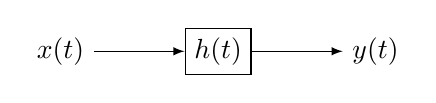
\begin{tikzpicture}
	       \draw[] (0,0) node (a) {$x(t)$} ++(2,0) node[draw=black] (b) {$h(t)$}  ++(2,0) node (c) {$y(t)$};
	       \draw[-latex]   (a) edge (b) (b) edge (c) ;
        \end{tikzpicture}
    \end{example}
    \pause
    \begin{align*}
      h(t) &= \delta(t-t_0)\\
      H(j\omega) &= e^{-j\omega t_0}\\
      Y(j\omega) &=  H(j\omega)  X(j\omega)\\
      &= e^{-j\omega t_0} X(j\omega)\\
    \end{align*}
\end{frame}

\begin{frame}
    \begin{example}
        What is the frequency response of the differentiator?
    \end{example}
    \pause
    The input output relationship of the differentiator is
    \begin{equation*}
        y(t) = \frac{dx(t)}{dt}.
    \end{equation*}
    From the differentiation property
    \pause
    \begin{equation*}
        Y(j\omega) = j\omega X(j\omega).
    \end{equation*}
    \pause
    Consequently, the frequency response of the differentiator is
    \begin{equation*}
        H(j\omega) = j\omega.
    \end{equation*}
\end{frame}


\begin{frame}
    \begin{example}
        Consider the response of an LTI system with impulse response
        \begin{equation*}
            h(t) = e^{-at}u(t), \quad a>0,
        \end{equation*}
        to the input signal
        \begin{equation*}
            x(t) = e^{-bt}u(t), \quad b>0.
        \end{equation*}
        Rather than computing $y(t) = x(t) \ast h(t)$ directly, find $y(t)$ by transfroming the problem into the frequency domain.
    \end{example}
\end{frame}

\begin{frame}
    \mode<beamer>
    {
        \begin{equation*}
            X(j\omega) = \frac{1}{b+j\omega}
        \end{equation*}
        \pause
        \begin{equation*}
            X(j\omega) = \frac{1}{a+j\omega}
        \end{equation*}
        \pause
        Therefore,
        \begin{equation*}
            Y(j\omega) = \frac{1}{(a+j\omega)(b+j\omega)}
        \end{equation*}
        To determine the output $y(t)$, we wish to obtain the inverse transform of $Y(j\omega)$. This is most simply done by expanding $Y(j\omega)$ in a partial-fraction expansion.
    }
\end{frame}

\begin{frame}
    \mode<beamer>
    {
        \begin{equation*}
            Y(j\omega) = \frac{A}{a+j\omega} + \frac{B}{b+j\omega}
        \end{equation*}
        \pause
        $b \neq a$
        \begin{equation*}
            A = \frac{1}{b-a} = -B,
        \end{equation*}
        \begin{equation*}
            Y(j\omega) = \frac{1}{b-a}\left[\frac{1}{a+j\omega} - \frac{1}{b+j\omega}\right]
        \end{equation*}
        \pause
        By inspection
        \begin{equation*}
            y(t) = \frac{1}{b-a}\left[ e^{-at}u(t) - e^{-bt}u(t)\right].
        \end{equation*}
    }
\end{frame}


\begin{frame}
    \mode<beamer>
    {
        For the case $a=b$,
        \begin{equation*}
            Y(j\omega) = \frac{1}{(a+j\omega)^2}.
        \end{equation*}
        \pause
        Recognizing this as
        \begin{equation*}
            \frac{1}{(a+j\omega)^2} = j\frac{d}{d\omega}\left[\frac{1}{a+j\omega}\right],
        \end{equation*}
        we can use the dual of the differentiation property,
        \begin{equation*}
            e^{-at}u(t) \overset{\mathcal{F}}{\longleftrightarrow} \frac{1}{a+j\omega}
        \end{equation*}
        \begin{equation*}
            te^{-at}u(t) \overset{\mathcal{F}}{\longleftrightarrow} j\frac{d}{d\omega}\left[\frac{1}{a+j\omega}\right] = \frac{1}{(a+j\omega)^2},
        \end{equation*}
        and consequently,
        \begin{equation*}
            y(t) = te^{-at}u(t).
        \end{equation*}
    }
\end{frame}



\begin{frame}{Multiplication Property}
    The convolution property states that convolution in \alert{time} domain corresponds to multiplication in \alert{frequency} domain. Because of the duality between time and frequency domains, we would expect a dual property also to hold (i.e., that multiplication in the time domain corresponds to convolution in the frequency domain). Specifically,

    \begin{equation*}
        r(t) = s(t)p(t) \overset{\mathcal{F}}{\longleftrightarrow} R(j\omega) = \frac{1}{2\pi}[S(j\omega)\ast P(j\omega)].
    \end{equation*}

    Multiplication of one signal by another can be thought of as using one signal to scale or \alert{modulate} the amplitude of the other. Consequently, the multiplication of two signals is often referred to as \alert{amplitude modulation}. For this reason, this equation is sometime referred to as the \alert{modulation property}.
\end{frame}

\begin{frame}[plain]
    \begin{example}
        Let $s(t)$ be a signal whose spectrum is depicted in the figure below. Also consider the signal
        \begin{equation*}
            p(t) = \cos\omega_0 t.
        \end{equation*}
        Show the spectrum of $r(t) = s(t)p(t)$.

        \begin{figure}
          \centering
          \begin{tikzpicture}[scale=0.6, every node/.append style={text=black, font=\scriptsize}]
	\begin{scope}
		\def\xmin{-8}
		\def\xmax{8}
		\def\ymin{0}
		\def\ymax{4}
		
		\draw[-latex] (\xmin, 0) -- (\xmax, 0) node[anchor=west] {$\omega$};
		\draw[-latex] (0, \ymin) -- (0, \ymax) node[anchor=south] {$S(j\omega)$};
		\node at (-1.5,0) [anchor=north] {$-\omega_1$};
		\node at (1.5,0) [anchor=north] {$\omega_1$};		
		
		\node at (0,2.5) [anchor=south east] {$A$};
		\draw  plot[smooth, tension=.2, thick, scale=0.5] coordinates {(-3,0) (-2.5,2) (-2,3) (-0.5,5) (0,5.35) (0.5, 5) (2,3) (2.5,2) (3,0)};
	\end{scope}

\end{tikzpicture}
          \caption{Spectrum of signal $s(t)$.}\label{fi:signal_for_modulation}
        \end{figure}
    \end{example}
\end{frame}
\begin{frame}[plain]
    \mode<beamer>
    {
        \begin{figure}
          \centering
          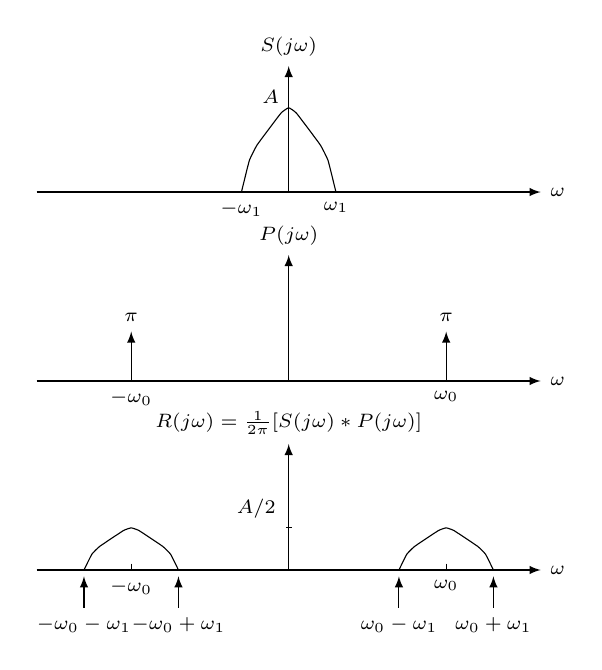
\begin{tikzpicture}[scale=0.4, every node/.append style={text=black, font=\scriptsize}]
	\begin{scope}
		\def\xmin{-8}
		\def\xmax{8}
		\def\ymin{0}
		\def\ymax{4}
		
		\draw[-latex] (\xmin, 0) -- (\xmax, 0) node[anchor=west] {$\omega$};
		\draw[-latex] (0, \ymin) -- (0, \ymax) node[anchor=south] {$S(j\omega)$};
		\node at (-1.5,0) [anchor=north] {$-\omega_1$};
		\node at (1.5,0) [anchor=north] {$\omega_1$};		
		
		\node at (0,2.5) [anchor=south east] {$A$};
		\draw  plot[smooth, tension=.2, thick, scale=0.5] coordinates {(-3,0) (-2.5,2) (-2,3) (-0.5,5) (0,5.35) (0.5, 5) (2,3) (2.5,2) (3,0)};
	\end{scope}
	
	\begin{scope}[yshift=-6cm]
		\def\xmin{-8}
		\def\xmax{8}
		\def\ymin{0}
		\def\ymax{4}
		
		\draw[-latex] (\xmin, 0) -- (\xmax, 0) node[anchor=west] {$\omega$};
		\draw[-latex] (0, \ymin) -- (0, \ymax) node[anchor=south] {$P(j\omega)$};
		\node at (-5,0) [anchor=north] {$-\omega_0$};
		\node at (5,0) [anchor=north] {$\omega_0$};		
		\draw[-latex] (-5,0) -- ++(0, pi/2) node [anchor=south] {$\pi$}; 		
		\draw[-latex] (5,0) -- ++(0, pi/2) node [anchor=south] {$\pi$}; 	
	\end{scope}
	
	\begin{scope}[yshift=-12cm]
		\def\xmin{-8}
		\def\xmax{8}
		\def\ymin{0}
		\def\ymax{4}
		
		\draw[-latex] (\xmin, 0) -- (\xmax, 0) node[anchor=west] {$\omega$};
		\draw[-latex] (0, \ymin) -- (0, \ymax) node[anchor=south] {$R(j\omega) = \frac{1}{2\pi}[S(j\omega)\ast P(j\omega)]$};
		\draw[] (-5,0.2) -- ++(0, -0.2);		
		\draw[] (5,0.2) -- ++(0, -0.2);	
		\node at (-5,0) [anchor=north] {$-\omega_0$};
		\node at (5,0) [anchor=north] {$\omega_0$};	
		\draw[latex-] (-5-1.5, -0.2) -- ++(0,-1) node[anchor=north] {$-\omega_0 - \omega_1$};
		\draw[latex-] (-5+1.5, -0.2) -- ++(0,-1) node[anchor=north] {$-\omega_0 + \omega_1$};
		\draw[latex-] (5-1.5, -0.2) -- ++(0,-1) node[anchor=north] {$\omega_0 - \omega_1$};
		\draw[latex-] (5+1.5, -0.2) -- ++(0,-1) node[anchor=north] {$\omega_0 + \omega_1$};		
		\draw  plot[smooth, tension=.2, thick, xscale=0.5, yscale=0.25, xshift= -10cm] coordinates {(-3,0) (-2.5,2) (-2,3) (-0.5,5) (0,5.35) (0.5, 5) (2,3) (2.5,2) (3,0)};
		\draw  plot[smooth, tension=.2, thick, xscale=0.5, yscale=0.25,  xshift=10cm] coordinates {(-3,0) (-2.5,2) (-2,3) (-0.5,5) (0,5.35) (0.5, 5) (2,3) (2.5,2) (3,0)};
		\draw (0.1, 5.35/4) -- ++(-0.2, 0) node [anchor=south east] {$A/2$};
	\end{scope}
	



\end{tikzpicture} 
          \caption{Fourier transform of $r(t) = s(t)p(t)$.}\label{fi:modulation_property}
        \end{figure}
    }


\end{frame}
